\id{МРНТИ 06.81.12}
\begin{articleheader}

\sectionwithauthors{А.Ф. Цеховой, Н.А. Некрасова, А.С. Жолтаева, Ж.Ж.Султанбекова, А.Ж. Турегельдинова}{AGILE-ПОДХОД К УПРАВЛЕНИЮ СОБЫТИЯМИ НЕДЕЛИ: ВВЕДЕНИЕ И ПРАКТИКА
ИСПОЛЬЗОВАНИЯ~МОДЕЛИ~АУСН}

{\bfseries \textsuperscript{1}А.Ф. Цеховой, \textsuperscript{2}Н.А.
Некрасова, \textsuperscript{1}А.С. Жолтаева, \textsuperscript{1}Ж.Ж.
Султанбекова\textsuperscript{\envelope }, \textsuperscript{1}А.Ж. Турегельдинова}
\end{articleheader}
\begin{affiliation}

\textsuperscript{1}Сатпаев Университет, Алматы, Казахстан,

\textsuperscript{2} ОЮЛ «Союз проектных менеджеров РК», Алматы,
Казахстан

\raggedright{\bfseries \textsuperscript{\envelope }}Корреспондент-автор:\href{mailto:z.sultanbekova@satbayev.university}{\nolinkurl{z.sultanbekova@satbayev.university}}
\end{affiliation}

В статье представлена модель Agile-управления событиями недели (АУСН),
основанная на технологии «Практика Agile-управления портфелем развития
организации» (ПАУПРО). Данная модель реализует продуктивный подход к
управлению взаимодействием членов команды управления организации,
интегрируя принципы Agile и методы проектного управления. Основное
внимание уделяется формированию продуктивных моделей управления,
основанных на принципах простоты и гибкости.

Ключевым аспектом АУСН является акцент на взаимодействии участников
команды, согласно первой ценности Agile: «Люди и взаимодействие важнее
процессов и инструментов», с уточнением о значении тех процессов,
которые обеспечивают это взаимодействие. В рамках модели реализуется
механизм оперативной самооценки эффективности управленческой
деятельности, через еженедельные оценки активности, значимости и
исполнительной дисциплины. Это способствует развитию саморефлексии,
самообучения и улучшению планирования взаимодействий с заинтересованными
сторонами.

Важно отметить, что система оценок в модели АУСН является инструментом
для саморазвития и , повышения управленческих компетенций. Цель
внедрения данной модели заключается в улучшении взаимодействия членов
управленческой команды, что способствует достижению высоких стандартов
качества и удовлетворенности клиентов, являясь важной частью стратегии
развития организации.

{\bfseries Ключевые слова:} Agile-управление, события недели, еженедельная
ретроспектива, продуктивное взаимодействие, управление развитием,
метрики оценки, активность планирования, дисциплина исполнения, качество
исполнения

\begin{articleheader}

{\bfseries АПТА ОҚИҒАЛАРЫН БАСҚАРУДАҒЫ AGILE ТӘСІЛІ: АОАБ МОДЕЛІН ЕНГІЗУ
ЖӘНЕ ҚОЛДАНУ ТӘЖІРИБЕСІ}

{\bfseries \textsuperscript{1}А.Ф. Цеховой, \textsuperscript{2}Н.А.
Некрасова, \textsuperscript{1}А.С. Жолтаева, \textsuperscript{1}Ж.Ж.
Сұлтанбекова\textsuperscript{\envelope },}

{\bfseries \textsuperscript{1}А.Ж. Турегельдинова}
\end{articleheader}
\begin{affiliation}

\textsuperscript{1}Сәтбаев Университеті, Алматы, Қазақстан,

\textsuperscript{2}«ҚР Жоба Менеджерлері Одағы» ЗТБ, Алматы, Қазақстан,

e-mail:
\href{mailto:z.sultanbekova@satbayev.university}{\nolinkurl{z.sultanbekova@satbayev.university}}
\end{affiliation}

Бұл мақалада «Апта оқиғаларын Agile-басқару моделі» (АОАБ) ұсынылған, ол
«Ұйымның даму портфелін Agile басқару практикасы» (ҰДМАБТ)
технологиясына негізделген. Бұл модель Agile принциптері мен жобалық
басқару әдістерін интеграциялай отырып, ұйымды басқару командасының
мүшелері арасындағы өзара әрекетті басқаруда өнімді тәсілді жүзеге
асырады. Негізгі назар өнімді басқару модельдерін қалыптастыруға
аударылған, олар қарапайымдылық пен икемділік принциптеріне негізделген.

АОАБ-дың негізгі аспектісі -- бұл Agile-дің «Адамдар мен өзара әрекет
процестер мен құралдардан маңызды» деген бірінші құндылығына сәйкес, сол
өзара әрекетті қамтамасыз ететін процестердің маңызын нақтылай отырып,
команда мүшелері арасындағы өзара әрекетке акцент қою болып табылады.
Модель шеңберінде апталық белсенділік, маңыздылық және орындаушылық
тәртіп бағалаулары арқылы басқарушылық қызметтің тиімділігін жедел
өзін-өзі бағалау механизмі жүзеге асырылады. Бұл өз-өзіне рефлексия,
өзін-өзі оқыту және мүдделі тараптармен өзара әрекеттестіктерді
жоспарлауды жақсартуға ықпал етеді.

АОАБ моделіндегі бағалау жүйесі өзін-өзі дамыту және басқарушылық
құзыреттерді жоғарылату үшін құрал болып табылатынын атап өту маңызды.
Бұл модельді енгізудің мақсаты басқару командасы мүшелерінің өзара
әрекеттесуін жақсарту болып табылады, ол жоғары сапа стандарттарына және
клиенттерді қанағаттандыруға қол жеткізуге ықпал етеді, бұл ұйымның даму
стратегиясының маңызды бөлігі болып табылады.

{\bfseries Түйін сөздер:} Agile-басқару, апта оқиғалары, апталық
ретроспектива, өнімді өзара әрекеттесу, дамуды басқару, бағалау
метрикалары, жоспарлау белсенділігі, орындау тәртібі, орындау сапасы.

\begin{articleheader}
{\bfseries AGILE APPROACH TO WEEKLY EVENT MANAGEMENT: INTRODUCTION AND
PRACTICE OF USING THE AMWE MODEL}

{\bfseries \textsuperscript{1}A.Ph. Tsekhovoy, \textsuperscript{2}N.A.
Nekrassova, \textsuperscript{1}A.S. Zholtayeva,
\textsuperscript{1}Zh.Zh. Sultanbekova\textsuperscript{\envelope },}

{\bfseries \textsuperscript{1}A.Zh. Turegeldinova}
\end{articleheader}
\begin{affiliation}

\textsuperscript{1}Satpayev University, Almaty, Kazakhstan,

\textsuperscript{1}Union of Project Managers of the Republic of
Kazakhstan, Almaty, Kazakhstan,

e-mail:
\href{mailto:z.sultanbekova@satbayev.university}{\nolinkurl{z.sultanbekova@satbayev.university}}
\end{affiliation}

The article presents the Agile Management Model for Weekly Events
(AMWE), based on the technology of "Agile Management Practices for
Organizational Development Portfolio" (AMPOD). This model implements a
productive approach to managing the interaction among members of the
organization's management team, integrating Agile principles and project
management methods. The primary focus is on forming productive
management models based on the principles of simplicity and flexibility.

A key aspect of the AMWE is its emphasis on the interaction among team
members, in accordance with the first value of Agile: "Individuals and
interactions over processes and tools," while clarifying the importance
of the processes that facilitate this interaction. Within the framework
of the model, a mechanism for operational self-assessment of management
effectiveness is implemented through weekly evaluations of activity,
significance, and executive discipline. This promotes the development of
self-reflection, self-learning, and improved planning of interactions
with stakeholders.

It is important to note that the evaluation system in the AMWE model
serves as a tool for self-development and enhancing managerial
competencies. The goal of implementing this model is to improve the
interaction among members of the management team, which contributes to
achieving high standards of quality and customer satisfaction,
representing an important part of the organization's development
strategy.

{\bfseries Keywords:} Agile-management, weekly events, weekly
retrospective, productive interaction, development management,
assessment metrics, planning activity, execution discipline, quality of
execution
\begin{multicols}{2}

{\bfseries Введение.} Современные организации, особенно малый и средний
бизнес (МСБ), сталкиваются с постоянными изменениями во внешней среде,
что требует от них гибкости, адаптивности и быстрой реакции на вызовы
{[}1,2{]}. Традиционные методы управления проектами, ориентированные на
детальное планирование и жесткое следование процессам, часто оказываются
недостаточными для удовлетворения этих требований. В условиях динамичных
изменений возникает необходимость внедрения гибких методов управления,
позволяющих организациям оперативно адаптироваться к изменяющимся
условиям {[}3{]}.

Одним из таких методов является Agile-управление, которое успешно
применяется в разработке программного обеспечения, а в последние годы
активно внедряется в различных секторах экономики. Принципы
Agile-методологии позволяют улучшить взаимодействие между членами
команды, повысить их вовлеченность и оперативно реагировать на
изменения. Однако использование Agile-технологий в управлении событиями
и задачами внутри организаций, особенно в контексте МСБ, требует
дальнейшего изучения и адаптации под конкретные реалии {[}4-6{]}.

В рамках данного исследования предлагается модель
{\bfseries Agile-управления событиями недели (АУСН)}, которая разработана с
учетом особенностей работы организаций малого и среднего бизнеса в
Казахстане. Эта модель направлена на улучшение управляемости организации
через эффективное планирование и реализацию еженедельных событий, что
позволяет добиться большей производительности, гибкости и устойчивости в
условиях постоянно меняющихся бизнес-реалий.

Целью данной работы является анализ и внедрение модели АУСН, основанной
на принципах Agile, для повышения эффективности управления портфелем
развития организаций МСБ. В статье рассматриваются теоретические и
практические аспекты использования модели АУСН, а также её влияние на
производительность и управленческую деятельность руководителей.

Исследование проведено в рамках научного проекта, направленного на
разработку продуктивных моделей управления портфелем развития
организаций малого и среднего бизнеса Казахстана, что делает данную тему
актуальной в контексте растущего спроса на гибкие управленческие
решения.

{\bfseries Материалы и методы.~} В данном исследовании для разработки и
анализа продуктивности модели АУСН применен широкий спектр научных
методов, обеспечивающих глубокое понимание и интеграцию концепций Agile
и современных подходов к управлению.

Для комплексного анализа и оценки эффективности модели АУСН использованы
следующие методы:

\begin{itemize}
\item
  \emph{Библиографический анализ}: оценка существующих исследований и
  публикаций, касающихся Agile-управления и состояния потока, а также их
  влияния на продуктивность и благополучие руководителей.
\item
  \emph{Обобщение, сравнение и синтез}: интеграция различных
  теоретических и практических подходов для формирования целостной
  модели управления.
\item
  \emph{Классификация и категоризация}: исследование факторов, влияющих
  на успешное внедрение модели АУСН, а также их воздействие на
  производительность и удовлетворенность руководителей.
\item
  \emph{Экспертная оценка}: сбор качественной информации от специалистов
  и руководителей, применяющих Agile-методы и концепции потока.
\item
  \emph{Методы наблюдения с активным участием}: сбор данных о реализации
  модели АУСН в реальных условиях, включая наблюдение за процессами и
  взаимодействиями в командах.
\end{itemize}

\emph{Принципы и подходы}

При разработке эффективных моделей управления, включая модель АУСН,
применяется один из ключевых принципов Agile --- «простота --- это
искусство максимизации объема работы, которую не нужно выполнять». Этот
принцип помогает сосредоточиться на важнейших аспектах управления и
избегать ненужных сложностей {[}7{]}.

В исследовании также учитываются идеи Джима Коллинза {[}8{]} и принципы
Agile. Эффективное развитие организации достигается, когда лидер
стремится к пятому уровню зрелости, формирует комплементарную команду,
способную объективно оценивать ситуацию, и внедряет
проектно-ориентированную систему управления. Кроме того, вносятся
поправки к ценностям Agile: «Люди и взаимодействия важнее процессов и
инструментов, если только они не способствуют этому взаимодействию».

Для оценки развития руководителей и эффективности модели АУСН выбраны
метрики: «работа», «быт», «здоровье», «досуг» и «саморазвитие». Эти
метрики позволяют всесторонне оценивать влияние модели на различные
аспекты жизни руководителей {[}9{]}.

\emph{База исследования}

Основной базой для исследования служат Союз проектных менеджеров
Республики Казахстан (СПМ РК), консалтинговая компания и предприятия
малого и среднего бизнеса (МСБ) города Алматы. Эти организации
предоставляют широкий спектр решений в области проектного, операционного
и стратегического менеджмента, основываясь на многолетнем опыте. Они
служат примерами успешного применения управленческих методов и создания
эффективной базы знаний, что позволяет оценить и адаптировать модель
АУСН в реальных условиях.

Таким образом, использование разнообразных методов и подходов
обеспечивает всесторонний анализ и разработку модели АУСН, направленной
на улучшение управления и благополучия руководителей в условиях
современных вызовов и изменений.

{\bfseries Результаты и обсуждение.}~ Модель АУСН, основанная на технологии
«Практика Agile-управления портфелем развития организации» (ПАУПРО),
представляет собой продуктивный подход к управлению развитием
организации, который интегрирует принципы Agile и методы проектного
управления как комплексного и универсального инструмента.

Основой ПАУПРО является совмещение трёх фаз развития и пяти доменов
исполнения, что позволяет эффективно управлять портфелем проектов,
обеспечивая гибкость и адаптивность.

Диаграмма Исикавы (или диаграмма причинно-следственных связей) может
быть мощным инструментом для анализа причин успешных или неуспешных
результатов в рамках модели АУСН. В контексте формирования ключевых
результативных индикаторов (КРI) через еженедельные ретроспективы, мы
можем использовать основные факторы для анализа причинно-следственных
связей:

\begin{enumerate}
\def\labelenumi{\arabic{enumi}.}
\item
  {\bfseries Процессы}:
\end{enumerate}

\begin{itemize}
\item
  Включают основные этапы, процессы и процедуры выполнения графика
  событий недели, такие как планирование, оценка задач, реализация и
  мониторинг.
\item
  Примеры факторов: неполное понимание требований, нечеткое планирование
  времени, неэффективные внутренние и внешние коммуникации,
  непродуктивное выполнение задач.
\end{itemize}

\begin{enumerate}
\def\labelenumi{\arabic{enumi}.}
\setcounter{enumi}{1}
\item
  {\bfseries Люди}:
\end{enumerate}

\begin{itemize}
\item
  Здесь рассматриваются участники процесса, их роли, ответственности и
  навыки, которые могут существенно влиять на результативность.
\item
  Примеры факторов: четко не обозначены роли и обязанности, конфликты
  между членами команды, недостаток необходимых навыков и компетенций.
\end{itemize}

\begin{enumerate}
\def\labelenumi{\arabic{enumi}.}
\setcounter{enumi}{2}
\item
  {\bfseries Технологии и инструменты}:
\end{enumerate}

\begin{itemize}
\item
  Охватывает инструменты и технологии, используемые для управления
  процессами и коммуникациями в рамках АУСН.
\item
  Примеры факторов: несовместимость инструментов, недостаточная
  автоматизация процессов, проблемы с доступом к необходимым ресурсам.
\end{itemize}

\begin{enumerate}
\def\labelenumi{\arabic{enumi}.}
\setcounter{enumi}{3}
\item
  {\bfseries Правила и процедуры}:
\end{enumerate}

\begin{itemize}
\item
  Это включает правила, стандарты и процедуры, регулирующие выполнение
  задач и процессов.
\item
  Примеры факторов: нечеткость в процессах управления изменениями,
  сложность в применении стандартов качества, несоответствие внутренних
  процедур текущим требованиям.
\end{itemize}

\begin{enumerate}
\def\labelenumi{\arabic{enumi}.}
\setcounter{enumi}{4}
\item
  {\bfseries Метрики}:
\end{enumerate}

\begin{itemize}
\item
  Оцениваются ключевые метрики, используемые для измерения эффектиность
  планирования, дисциплина исполнения и качество проведения событий
  недели.
\item
  Примеры факторов: неадекватные метрики для измерения успеха,
  недостоверность данных метрик, отсутствие системы мониторинга и
  анализа.
\end{itemize}

\begin{enumerate}
\def\labelenumi{\arabic{enumi}.}
\setcounter{enumi}{5}
\item
  {\bfseries Окружающая среда}:
\end{enumerate}

\begin{itemize}
\item
  Учитываются внешние факторы, такие как изменения в бизнес-среде,
  требования клиентов, конкурентные условия и законодательные нормы.
\item
  Примеры факторов: изменения в требованиях клиентов, экономические
  изменения, изменения в законодательстве (см. рис. 1).
\end{itemize}
\end{multicols}

\begin{figure}[H]
	\centering
	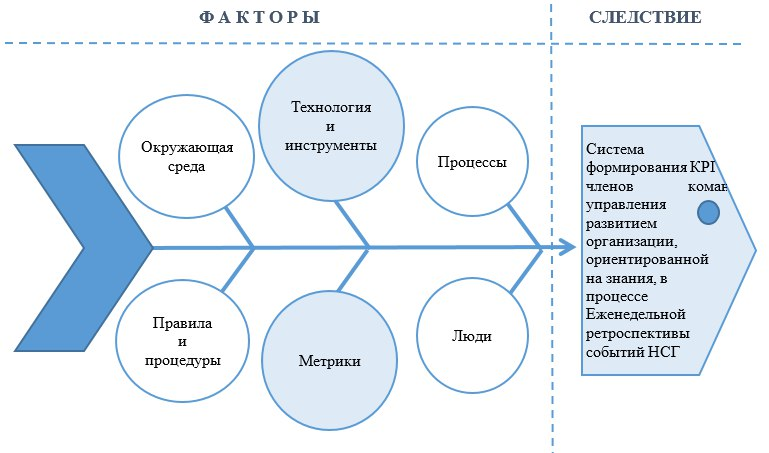
\includegraphics[width=0.8\textwidth]{media/ekon/image3.1}
	\caption*{Рис. 1 - Диаграмма Исикавы}
\end{figure}

\begin{multicols}{2}

Данный подход позволил систематизировать и визуализировать ключевые
факторы, влияющие на успех проекта, и помог команде Agile более
эффективно анализировать и улучшать процессы и процедуры на основе
полученных данных.

Продуктивная модель АУСН предполагает установление взаимодействия между
членами команды в соответствии с первой ценностью Agile-управления:
«Люди и взаимодействие важнее процессов и инструментов». Мы вводим
уточнение: «кроме тех, которые обеспечивают это взаимодействие». Это
дополнение отражает основную направленность нашей технологии.

В рамках разрабатываемой модели АУСН акцент сделан на создание механизма
оперативной самооценки управленческой деятельности. Каждая неделя
начинается со сводной оценки активности, исполнительной дисциплины и
качества реализованных мероприятий за прошедшую неделю. После этого
каждый участник команды, включая генерального директора (СЕО) и
топ-менеджеров, проводит самооценку достигнутых результатов. Это
способствует развитию саморефлексии, самообучения, более эффективному
планированию и повышению качества взаимодействий с заинтересованными
сторонами.

Основное отличие данной модели состоит в том, что она направлена на
саморазвитие членов команды управления. АУСН представляет собой
инструмент для личного развития и повышения профессиональных
компетенций, что выражает принципиальную новизну подхода по отношению к
оценке эффективности управленческой деятельности.

Цель внедрения модели АУСН заключается в улучшении взаимодействия членов
команды управления, ориентированной на достижение высоких стандартов
качества и удовлетворение растущих запросов клиентов. Это является
неотъемлемой частью стратегии развития организации.

Переход к Agile-методологии требует использования новых показателей и
метрик для оценки эффективности команды и достижения целей организации.
Важно выявить такие метрики, которые будут значимы как для команды, так
и для руководства, и которые будут ориентированы на получение ценности
организации {[}10{]}. В рамках разработки модели АУСН авторы стремились
измерить такие аспекты, как инициативность, эффективность планирования,
качество работы сотрудников, и связать эти измерения с системой
мотивации.

Цель - создать методологию, позволяющую объективно оценивать и улучшать
взаимодействие и производительность в организации, ориентированной на
знания.

Компонентами модели АУСН являются:

\begin{itemize}
\item
  Календарь года;
\item
  График событий недели (ГСН);
\item
  Расписание событий дня (РСД);
\item
  Система оценки;
\item
  Система мотивации.
\end{itemize}

Основой модели является формирование календаря года орагнизации, что
позволяет планировать работу и координировать усилия всех участников
проектов, программ и мероприятий. Этот календарь встраивается в
управленческие процессы компании и служит основой для планирования
результатов (продуктов) и решения приоритетных задач. Такой подход
обеспечивает структурированность работы и помогает достигать
поставленных целей в срок.

Обязательным компонентом модели являются график событий недели (ГСН)
\emph{(см. рис.2)}.
\end{multicols}

\begin{figure}[H]
	\centering
	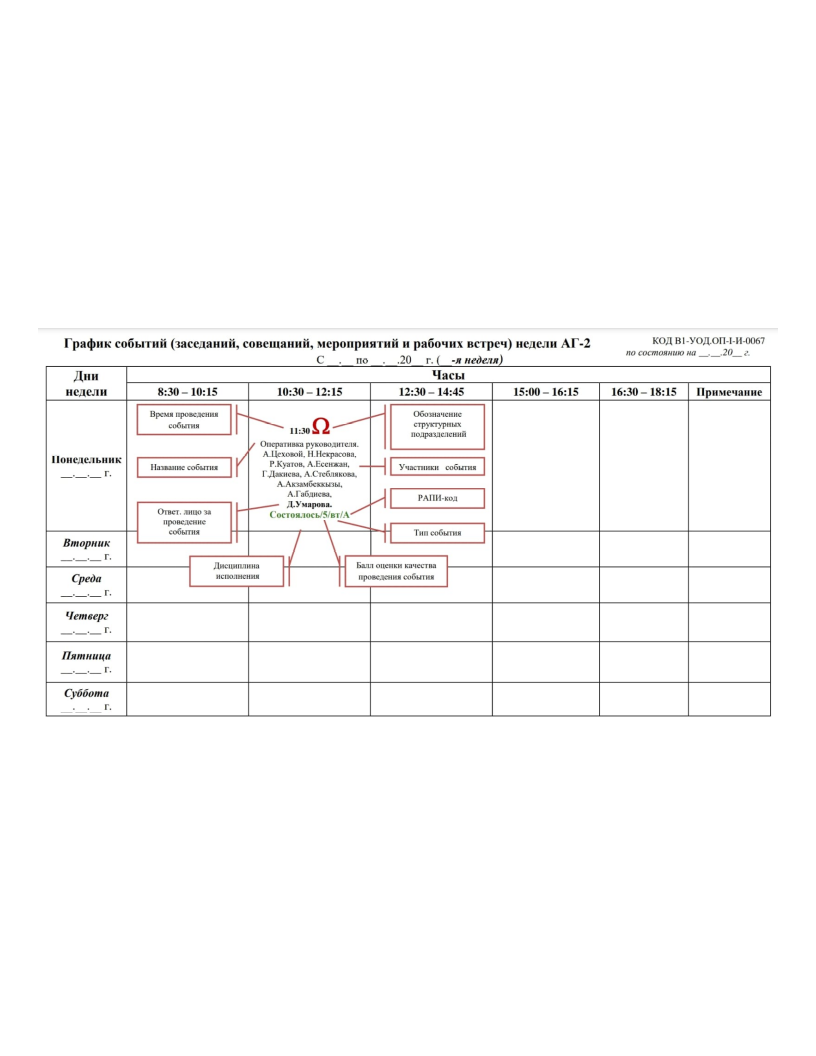
\includegraphics[width=0.8\textwidth]{media/ekon/image2}
	\caption*{Рис.- 2 Шаблон Графика событий недели (ГСН)}
\end{figure}

\begin{multicols}{2}

График событий недели (ГСН) формируется командой управления развитием
организации исходя из документов: «Календарь года», «Вопросы развития
организации», «Перечень не состоявшихся и перенесенных событий» и
«Вопросы развития структурных подразделений». График содержит следующие
данные:

\begin{itemize}
\item
  обозначения структурных подразделений латинскими буквами (литера);
\item
  наименования событий;
\item
  место проведения;
\item
  время проведения;
\item
  ФИО ответственного лица за организацию и проведение мероприятия;
\item
  ФИО участников;
\item
  отметка об исполнении;
\item
  балл оценки качества исполнения;
\item
  тип события;
\item
  РАПИ-код.
\end{itemize}

Офис-менеджер мониторит график событий в течение недели и при
необходимости оказывает организационно-техническую поддержку участникам.
Исходя из оценки руководства и ответственного лица, офис-менеджер по
каждому проведенному событию присваивает баллы дисциплины и качества
исполнения.

На основе графика событий недели каждый день формируется «Расписание
событий дня» (РСД)\emph{.} РСД позволяет обеспечитьт актуализацию планов
и координацию действий всех участников на ежедневной основе.

Таким образом, модель АУСН интегрирует стратегическое и оперативное
планирование, контроль, оценку и мотивацию в единый управленческий
процесс, направленный на повышение эффективности взаимодействия и
производительности в организации, ориентированной на знания.

Особенности этого управленческого процесса заключается в следующем:

а) проводится первым руководителем;

б) в оперативном совещании участвуют руководители структурных
подразделений (которые, как правило, и входят в состав команды
управления развитием организации);

в) день проведения -- понедельник - первый рабочий день недели;

г) время проведения -- 11 часов дня (дается возможность участникам
подготовиться к началу совещания);

д) совещание проводится с визуализацией отчета по ГСН за предыдущую
неделю и ГСН на предстоящую неделю на экране в офлайн формате или на
компьютере при онлайн подключении с использованием Zoom или других
приложений.

Ключевые этапы процесса еженедельной ретроспективы включают:

\begin{itemize}
\item
  Мониторинг ГСН в течение недели;
\item
  Оценка и анализ событий в ГСН за предыдущую неделю;
\item
  Формирование и актуализацию ГСН на текущую неделю;
\item
  Обсуждение результатов событий, их влияния на реализацию приоритетов и
  стратегии развития организации, потенциальные возможности (по РАПИ
  коду), ,
\item
  Актуализацию календаря года, планирование событий на предстоящую
  неделю.
\end{itemize}

Ключевыми участниками данного процесса являются: топ-менеджеры,
руководители структурных подразделений и офис-менеджер. Эти оперативные
совещания направлены на эффективное использование коллективных ресурсов.

Офис-менеджер совместно с менеджером по управлению знаниями готовит
анализ для оценки исполнения намеченных и фактически выполненных
событий, мероприятий, встреч, внутренних процессов. Выходом данного
анализа является оценка полноты и качества исполнения запланированных
событий прошедшей недели и формирование плана действий на предстоящую
неделю. Одновременно оценивается активность взаимодействия и
сравнительный прирост интеллектуальной активности через анализ
Генерального реестра информационных объектов (ГРИО).

Одной из ключевых задач еженедельной Agile-оперативки, проводимой первым
руководителем по модели АУСН, является мониторинг влияния текущих
событий на статус зарегистрированных возможностей и выявление
предпосылок для регистрации новых возможностей. В настоящее время авторы
сосредоточены на оптимизации процесса регистрации активности
топ-менеджеров, касающейся инициации событий, включаемых в НСГ, и оценки
дисциплины и качества исполнения.

После завершения настройки этих параметров, планируется интеграция
процедуры рассмотрения вопросов, внесенных в матрицу регистрации
возможностей, в еженедельные оперативные совещания. Для топ-менеджеров и
руководителей структур полезно при подготовке к оперативному совещанию
рассмтривать статус возможностей на предмет планирования встреч и
мероприятий для их реализации.

Каждый субъект управления обозначает выходы прошедшей недели, и
планируемых выходов на предстоящую неделю.

Данный подход поможет проанализировать то, как командные взаимодействия,
подверженные влиянию внешних факторов, соотносятся с внутренними
факторами организации и активами ее внутренних процессов.

Итоговое резюме руководителя на оперативном совещании представляет собой
ключевой компонент процесса управления, направленного на систематизацию
и оценку результатов работы, выявление перспектив для развития и
разрешение проблемных аспектов внутри организации. В резюме должны быть
«снивелированы» дискуссионные моменты, которые могут возникать по ходу
обсуждения и изложены «точки приложения усилий» членов команды
управления на предстоящий период. Резюме служит инструментом для
обобщения итогов оперативного совещания, определения направлений для
дальнейшего улучшения и обеспечения согласованности действий членов
команды управления. Резюме состоит из следующих разделов:

1. Выходы рабочей недели (outputs)

«Выходы рабочей недели» (outputs) обозначают конкретные результаты и
достижения, полученные в рамках запланированных мероприятий за отчетный
период. Эти результаты могут включать завершенные задачи, подготовленные
отчеты, проведенные мероприятия и достигнутые цели. Оценка выходов
позволяет определить продуктивность работы и соответствие деятельности
намеченным планам.

2. Точки роста

«Точки роста» обозначают новые возможности и области для улучшения,
выявленные в ходе работы за неделю. Они касаются как внутренних
процессов, так и внешних факторов, таких как изменения на рынке или
новые потребности клиентов. Анализ точек роста позволяет выявить
перспективные направления для развития и оптимизации.

3. Точки дискомфорта

«Точки дискомфорта» обозначают аспекты работы, которые вызывают
неудовлетворенность или проблемы у сотрудников. Эти точки могут быть
связаны как с внутренними процессами, так и с внешними факторами.
Определение и анализ точек дискомфорта позволяют быстро реагировать на
возникающие проблемы и предотвращать их эскалацию. Анализ точек
дискомфорта позволяет улучшить рабочие условия, повысить мотивацию
сотрудников и создать более эффективную рабочую среду.

Систематизация данных в заключительносм резюме помогает обеспечить
ясность в управлении, согласованность действий и стратегическую
направленность на достижение поставленных целей.

Таким образом, процесс еженедельной ретроспективы событий недели АГ-2 в
процессе Agile-управления событиями недели обеспечивает систематический
подход к оценке и улучшению взаимодействий внутри организации. Это
способствует более целенаправленной и эффективной работе, улучшению
управления временем и ресурсами, а также повышению конкурентоспособности
организации.

Информационно-техническая поддержка проведения оперативного совещания
базируется на разработанном шаблоне документа «Информация о выполнении
ГСН» (\emph{см. рис. 3}), который визуализирует оценку активности,
дисциплины и качества исполнения и ценности полученных выходов (out-put)
для развития организации.
\end{multicols}

\begin{figure}[H]
	\centering
	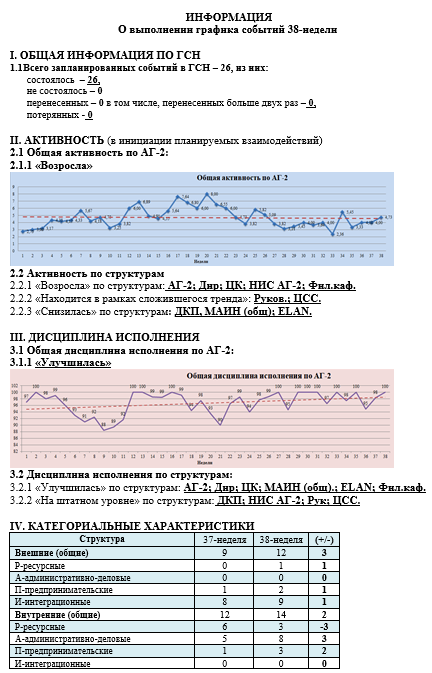
\includegraphics[width=0.8\textwidth]{media/ekon/image3}
	\caption*{Рис.- 3 Пример документа «Информация о выполнении ГСН»}
\end{figure}


Для заполнения документа «Информация о выполнении ГСН» офис-менеджер в
течение недели заполняет форму первичного отчета в excel (см. табл. 1).

{\bfseries Таблица 1 Форма первичного отчета о выполнении ГСН в excel}

% \begin{longtable}[]{@{}
%   >{\raggedright\arraybackslash}p{(\columnwidth - 28\tabcolsep) * \real{0.2699}}
%   >{\raggedright\arraybackslash}p{(\columnwidth - 28\tabcolsep) * \real{0.0596}}
%   >{\raggedright\arraybackslash}p{(\columnwidth - 28\tabcolsep) * \real{0.0745}}
%   >{\raggedright\arraybackslash}p{(\columnwidth - 28\tabcolsep) * \real{0.0744}}
%   >{\raggedright\arraybackslash}p{(\columnwidth - 28\tabcolsep) * \real{0.0447}}
%   >{\raggedright\arraybackslash}p{(\columnwidth - 28\tabcolsep) * \real{0.0745}}
%   >{\raggedright\arraybackslash}p{(\columnwidth - 28\tabcolsep) * \real{0.0447}}
%   >{\raggedright\arraybackslash}p{(\columnwidth - 28\tabcolsep) * \real{0.0448}}
%   >{\raggedright\arraybackslash}p{(\columnwidth - 28\tabcolsep) * \real{0.0448}}
%   >{\raggedright\arraybackslash}p{(\columnwidth - 28\tabcolsep) * \real{0.0448}}
%   >{\raggedright\arraybackslash}p{(\columnwidth - 28\tabcolsep) * \real{0.0447}}
%   >{\raggedright\arraybackslash}p{(\columnwidth - 28\tabcolsep) * \real{0.0446}}
%   >{\raggedright\arraybackslash}p{(\columnwidth - 28\tabcolsep) * \real{0.0447}}
%   >{\raggedright\arraybackslash}p{(\columnwidth - 28\tabcolsep) * \real{0.0447}}
%   >{\raggedright\arraybackslash}p{(\columnwidth - 28\tabcolsep) * \real{0.0447}}@{}}
% \toprule\noalign{}
% \begin{minipage}[b]{\linewidth}\raggedright
% \_n-НЕДЕЛЯ
% \end{minipage} &
% \multicolumn{6}{>{\raggedright\arraybackslash}p{(\columnwidth - 28\tabcolsep) * \real{0.3725} + 10\tabcolsep}}{%
% \begin{minipage}[b]{\linewidth}\raggedright
% Количество событий
% \end{minipage}} &
% \multicolumn{4}{>{\raggedright\arraybackslash}p{(\columnwidth - 28\tabcolsep) * \real{0.1790} + 6\tabcolsep}}{%
% \begin{minipage}[b]{\linewidth}\raggedright
% Внутренние
% \end{minipage}} &
% \multicolumn{4}{>{\raggedright\arraybackslash}p{(\columnwidth - 28\tabcolsep) * \real{0.1786} + 6\tabcolsep}@{}}{%
% \begin{minipage}[b]{\linewidth}\raggedright
% Внешние
% \end{minipage}} \\
% \midrule\noalign{}
% \endhead
% \bottomrule\noalign{}
% \endlastfoot
% Структурs & Запланированные & Состоявшиеся & Не состоявшиеся &
% Перенесенные & Перенесенные

% более 2-х раз & Потерянные & Р & А & П & И & Р & А & П & И \\
% АГ-2 ({\bfseries Ω}) & & & & & & & & & & & & & & \\
% Руководитель ({\bfseries Ρ}) & & & & & & & & & & & & & & \\
% Дирекция СПМ РК ({\bfseries Ν}) & & & & & & & & & & & & & & \\
% ДКП ({\bfseries Δ}) & & & & & & & & & & & & & & \\
% Центр Консалт ({\bfseries K}) & & & & & & & & & & & & & & \\
% Центр сертиф. ({\bfseries ϛ}) & & & & & & & & & & & & & & \\
% МАИН (общая) ({\bfseries μ}) & & & & & & & & & & & & & & \\
% МАИН (устав.) ({\bfseries μ1}) & & & & & & & & & & & & & & \\
% МАИН (контр.) ({\bfseries μ2}) & & & & & & & & & & & & & & \\
% НИС АГ-2 ({\bfseries π}) & & & & & & & & & & & & & & \\
% ELAN ({\bfseries Σ}) & & & & & & & & & & & & & & \\
% Филиал МиМЭ ({\bfseries φ}) & & & & & & & & & & & & & & \\
% Итого по стуктурам & & & & & & & & & & & & & & \\
% \end{longtable}

\begin{multicols}{2}
После заполнения формы первичного отчета автоматически в сводной таблице
(в excel) формируются данные согласно разделам Информации о выполнении
ГСН.

Первый раздел содержит общую информацию по ГСН. Определяется количество
запланированных событий в ГСН, из них количество состоявшихся, не
состоявшихся, перенесенных, в том числе, перенесенных больше двух раз и
«потерянных».

Процессом «Еженедельная ретроспектива графика событий недели»
измеряется:

а) активность членов команды управления, включая СЕО (в баллах, исходя
из количества инициированных ими событий в НСГ), рисунок 3;

б) дисциплину исполнения запланированных событий (в баллах), рисунок 3;

в) качество исполнения (с учётом системы оценки «выходов» (outputs), в
баллах.

Эффективность этого процесса будет зависеть от факторов, неисследованных
на текущий момент, среди которых -- корректность метрик, используемых
для анализа выходов (outputs) недели и алгоритма формирования фокуса
действий на предстоящий период (как правило --неделя).

Модель АУСН реальной жизнедеятельности способствует формированию
Agile-мышления, прежде всего у субъекта управления высшего уровня, каким
является СЕО, а затем и у членов команды управления развитием и далее --
будет поддерживать динамику создания конкурентоспособного корпоративного
знания (как правило, в формализованном виде) {[}11{]}.

Интенсивное и качественное взаимодействие субъектов управления
способстует приросту корпоративных знаний. Чем больше коммуницируют
члены команды управления, тем продуктивнее компания {[}12{]}.

{\bfseries Выводы.~}Продуктивная модель Agile-управления событиями недели
(АУСН), основанная на технологии ПАУПРО, представляет собой
инновационный подход к управлению развитием организации. Ориентированная
на гибкость, адаптивность и эффективность, данная модель позволяет
интегрировать Agile-принципы с системой управления знаниями, что создаёт
уникальную основу для успешного роста и развития в условиях быстро
меняющегося бизнес-окружения.

АУСН позволяет организациям оперативно адаптироваться к рыночным
изменениям, эффективно реагировать на новые вызовы и возможности, а
также рационально использовать ресурсы. Систематический анализ и оценка
событий и мероприятий недели помогают команде управления принимать
обоснованные решения, способствующие достижению стратегических целей.

Применение модели АУСН способствует формированию предпринимательской
среды «Новой волны», где ключевыми факторами являются гибкость,
инновации и непрерывное обучение. Этот подход поддерживает развитие
малого бизнеса в Казахстане, предоставляя компаниям возможность успешно
конкурировать на рынке и расширять свои возможности.

Таким образом, модель АУСН является важным инструментом для организаций,
стремящихся к устойчивому развитию и конкурентным преимуществам в
современном бизнесе. Ее использование содействует созданию гибкой и
адаптивной корпоративной культуры, где инновации и знания играют
центральную роль в достижении успеха.

\emph{{\bfseries Финансирование.} Статья выполнена в рамках проекта НИР
АР14871548 «}\emph{Разработка} \emph{продуктивных моделей}
\emph{управления портфелем развития организаций малого и среднего
бизнеса для условий Казахстана на основе идей и принципов
Agile-технологий».}
\end{multicols}


\begin{center}
  {\bfseries Литература}
  \end{center}
  
  \begin{references}
1.Сазерленд Дж. Scrum. Революционный метод управления проектами/ Джефф
Сазерленд; пер. с англ. Марии Гескиной. - Москва: Манн, Иванов и Фербер,
2016.- 272 с.

ISBN 9785001465096

2.Адизес, И. Управление жизненным циклом корпораций / Ицхак Калдерон
Адизес; пер. с англ. В.Кузина. -- М.: Манн, Иванов и Фербер, 2014.- 512
с. ISBN 978-5-00057-151-4

3.Daraojimba E.Ch., Nwasike Chi.N., Adegbite A.O., Ezeigweneme Ch.A.,
Gidiagba J.O. Comprehensive review of Agile methodologies in project
management //
\href{https://www.researchgate.net/journal/Computer-Science-IT-Research-Journal-2709-0051?_tp=eyJjb250ZXh0Ijp7ImZpcnN0UGFnZSI6Il9kaXJlY3QiLCJwYWdlIjoicHVibGljYXRpb24iLCJwcmV2aW91c1BhZ2UiOiJfZGlyZWN0In19}{Computer
Science \& IT Research Journal}. - 2024.-Vol.5(1).- P.190-218. DOI
\href{http://dx.doi.org/10.51594/csitrj.v5i1.717}{10.51594/csitrj.v5i1.717}

4. Борисов Н.С. Применение методов Agile в управлении проектами //
Индустриальная экономика.-2021 -Vol.1.- P. 74-77. DOI
\href{https://doi.org/10.47576/2712-7559_2021_1_74}{10.47576/2712-7559\_2021\_1\_74}

5. Sudhakar Babu S. Trends in IT Project Management: Agile Methodologies
and Their Impact on Project Success // Journal of Recent Trends in
Computer Science and Engineering (JRTCSE). -2024.-Vol. 12(2). - P.
73-81. https://jrtcse.com

6.\href{https://www.researchgate.net/scientific-contributions/Haibo-Li-2290691805?_tp=eyJjb250ZXh0Ijp7ImZpcnN0UGFnZSI6Il9kaXJlY3QiLCJwYWdlIjoicHVibGljYXRpb24iLCJwcmV2aW91c1BhZ2UiOiJfZGlyZWN0In19}{Haibo
L.} Application and Practice of Agile Methods in Project Management //
\href{https://www.researchgate.net/journal/Journal-of-Applied-Economics-and-Policy-Studies-2977-571X?_tp=eyJjb250ZXh0Ijp7ImZpcnN0UGFnZSI6Il9kaXJlY3QiLCJwYWdlIjoicHVibGljYXRpb24iLCJwcmV2aW91c1BhZ2UiOiJfZGlyZWN0In19}{Journal
of Applied Economics and Policy Studies}. -- 2024. Vol. 7(1).- P .71-74
DOI
\href{http://dx.doi.org/10.54254/2977-5701/7/2024076}{10.54254/2977-5701/7/2024076}

7.Agile: Практическое руководство / {[}пер. с англ.{]} --- М.:
Издательство «Олимп--Бизнес». -- 2019.-182 с. ISBN 978-5-9693-0403-1
(рус.) ISBN 978-1-62825-418-1 (англ.)

8. Коллинз Д. От хорошего к великому / Д. Коллинз -- М.: Манн, Иванов и
Фербер, 2017. -- 378 с.пер.с анг.

9.Цеховой А.Ф., Степанов А.В., Некрасова Н.А., Жолтаева А.С.
Профессиональные управленческие знания как фактор ускоренного развития
Казахстана // Вестник университета «Туран».-2023.- Vol.3.- С. 75-89.
\href{https://doi.org/10.46914/1562-2959-2023-1-3-75-89}{DOI10.46914/1562-2959-2023-1-3-75-89}

10.Хаббард Д. Как измерить все, что угодно. Оценка стоимости
нематериального в бизнесе / Дуглас У. Хаббард; пер. с англ. Е.
Пестеревой. -- М.: ЗАО «Олимп-Бизнес», 2009. -- 320 с.

11. \href{https://www.emerald.com/insight/search?q=Mahmoud\%20Mohammad\%20Migdadi}{Migdadi
M.M.} Knowledge management processes: innovation capability and
organizational performance //
\href{https://www.emerald.com/insight/publication/issn/1741-0401}{International
Journal of Productivity and Performance Management}. -- 2022. -- Vol.
71(1)- P.182-210. \href{https://doi.org/10.1108/ijppm-04-2020-0154}{DOI
10.1108/ijppm-04-2020-0154}

12.Цеховой А.Ф., Ли А., Азиева З. О роли организаций, ориентированных на
знания, в придании импульса развитию МСБ в Казахстане // Материалы
Международной научно-практической конференции КСТУ имени академика
З.Алдамжара. -- 2020. -- 224 с.
\end{references}

\begin{center}
{\bfseries References}
\end{center}

\begin{references}

1.Sazerlend Dzh. Scrum. Revoljucionnyj metod upravlenija proektami/
Dzheff Sazerlend; per. s angl. Marii Geskinoj. - Moskva: Mann, Ivanov i
Ferber, 2016.- 272 s. ISBN 9785001465096.

{[}in Russian{]}

2.Adizes, I. Upravlenie zhiznennym ciklom korporacij / Ichak Kalderon
Adizes; per. s angl. V.Kuzina. -- M.: Mann, Ivanov i Ferber, 2014.- 512
s. ISBN 978-5-00057-151{\bfseries -}4.{[}in Russian{]}

3.Daraojimba E.Ch., Nwasike Chi.N., Adegbite A.O., Ezeigweneme Ch.A.,
Gidiagba J.O. Comprehensive review of Agile methodologies in project
management //
\href{https://www.researchgate.net/journal/Computer-Science-IT-Research-Journal-2709-0051?_tp=eyJjb250ZXh0Ijp7ImZpcnN0UGFnZSI6Il9kaXJlY3QiLCJwYWdlIjoicHVibGljYXRpb24iLCJwcmV2aW91c1BhZ2UiOiJfZGlyZWN0In19}{Computer
Science \& IT Research Journal}. - 2024.-Vol.5(1).- P.190-218. DOI
\href{http://dx.doi.org/10.51594/csitrj.v5i1.717}{10.51594/csitrj.v5i1.717}

4. Borisov N.S. Primenenie metodov Agile v upravlenii proektami //
Industrial' naja jekonomika.-2021 -Vol.1.- P. 74-77. DOI
10.47576/2712-7559\_2021\_1\_74.{[}in Russian{]}

5. Sudhakar Babu S. Trends in IT Project Management: Agile Methodologies
and Their Impact on Project Success // Journal of Recent Trends in
Computer Science and Engineering (JRTCSE). -2024.-Vol. 12(2). - P.
73-81. https://jrtcse.com.{[}in Russian{]}

6.\href{https://www.researchgate.net/scientific-contributions/Haibo-Li-2290691805?_tp=eyJjb250ZXh0Ijp7ImZpcnN0UGFnZSI6Il9kaXJlY3QiLCJwYWdlIjoicHVibGljYXRpb24iLCJwcmV2aW91c1BhZ2UiOiJfZGlyZWN0In19}{Haibo
L.} Application and Practice of Agile Methods in Project Management //
\href{https://www.researchgate.net/journal/Journal-of-Applied-Economics-and-Policy-Studies-2977-571X?_tp=eyJjb250ZXh0Ijp7ImZpcnN0UGFnZSI6Il9kaXJlY3QiLCJwYWdlIjoicHVibGljYXRpb24iLCJwcmV2aW91c1BhZ2UiOiJfZGlyZWN0In19}{Journal
of Applied Economics and Policy Studies}.-2024. Vol. 7(1).- P .71-74.

DOI
\href{http://dx.doi.org/10.54254/2977-5701/7/2024076}{10.54254/2977-5701/7/2024076}.
{[}in Russian{]}

8. Kollinz D. Ot horoshego k velikomu / D. Kollinz - M.: Mann, Ivanov i
Ferber, 2017. -378 s. {[}in Russian{]}

9.Cehovoj A.F., Stepanov A.V., Nekrasova N.A., Zholtaeva A.S.
Professional' nye upravlencheskie znanija kak faktor
uskorennogo razvitija Kazahstana // Vestnik universiteta «Turan».-2023.-
Vol.3.- S. 75-89. DOI10.46914/1562-2959-2023-1-3-75-89.{[}in Russian{]}

10.Habbard D. Kak izmerit'{} vse, chto ugodno. Ocenka
stoimosti nematerial' nogo v biznese / Duglas U. Habbard;
per. s angl. E. Pesterevoj.- M.: ZAO «Olimp-Biznes», 2009.-320 s.

{[}in Russian{]}

11.
\href{https://www.emerald.com/insight/search?q=Mahmoud\%20Mohammad\%20Migdadi}{Migdadi
M.M.} Knowledge management processes: innovation capability and
organizational performance //
\href{https://www.emerald.com/insight/publication/issn/1741-0401}{International
Journal of Productivity and Performance Management}.- 2022.- Vol. 71(1)-
P.182-210. \href{https://doi.org/10.1108/ijppm-04-2020-0154}{DOI
10.1108/ijppm-04-2020-0154}

12.Cehovoj A.F., Li A., Azieva Z. O roli organizacij, orientirovannyh na
znanija, v pridanii impul' sa razvitiju MSB v Kazahstane
// Materialy Mezhdunarodnoj nauchno-prakticheskoj konferencii KSTU imeni
akademika Z.Aldamzhara. -2020.- S 224. {[}in Russian{]}
\end{references}

\begin{authorinfo}
\hspace{1em}\emph{{\bfseries Сведения об авторах}}

Цеховой А.Ф. {\bfseries -} д.т.н., профессор, Сатпаев Университет, Алматы,
Казахстан, e-mail: \href{mailto:tsaf@list.ru}{\nolinkurl{tsaf@list.ru}};

Некрасова Н.А. {\bfseries -} Союз проектных менеджеров Республики
Казахстан, Алматы, Казахстан, e-mail:
\href{mailto:info@spmrk.kz}{\nolinkurl{info@spmrk.kz}};

Жолтаева А.С. - PhD, Сатпаев Университет{\bfseries ,} Алматы, Казахстан,
e-mail:
\href{mailto:a_zholtayeva@mail.ru}{\nolinkurl{a\_zholtayeva@mail.ru}};

Султанбекова Ж.Ж. {\bfseries -} к.т.н., ассоциированный профессор, Сатпаев
Университет{\bfseries ,} Алматы, Казахстан, e-mail:
\href{mailto:z.sultanbekova@satbayev.university}{\nolinkurl{z.sultanbekova@satbayev.university}};

Турегельдинова А.Ж. - PhD, ассоциированный профессор, Сатпаев
Университет{\bfseries ,} Алматы, Казахстан, e-mail:
\href{mailto:a.turegeldinova@satbayev.university}{\nolinkurl{a.turegeldinova@satbayev.university}}.

\hspace{1em}\emph{{\bfseries Information about the authors}}

Tsekhovoy А.Ph{\bfseries . -} d.t.s., professor, Satbayev University,
Almaty, Kazakhstan, e-mail:
\href{mailto:tsaf@list.ru}{\nolinkurl{tsaf@list.ru}};

Nekrassova N.А. {\bfseries -} Union of Project Managers of the Republic of
Kazakhstan, Almaty, Kazakhstan, e-mail:
\href{mailto:info@spmrk.kz}{\nolinkurl{info@spmrk.kz}};

Zholtayeva А.S. - PhD, Satbayev University, Almaty, Kazakhstan, e-mail:
\href{mailto:a_zholtayeva@mail.ru}{\nolinkurl{a\_zholtayeva@mail.ru}};

Sultanbekova Zh.Zh. {\bfseries -} candidate of technical sciences Satbayev
University, , associate professor, Almaty, Kazakhstan, e-mail:
\href{mailto:z.sultanbekova@satbayev.university}{\nolinkurl{z.sultanbekova@satbayev.university}};

Turegeldinova А.Zh.-PhD, associate professor Satbayev University Almaty,
Kazakhstan, e-mail:

\href{mailto:a.turegeldinova@satbayev.university}{\nolinkurl{a.turegeldinova@satbayev.university}}.
\end{authorinfo}
